% \documentclass[answers]{exam}
\documentclass{exam}
\usepackage{listings}
\usepackage{inconsolata}
\usepackage{graphicx}

\lstset{language=Java,basicstyle=\ttfamily,showspaces=false,showstringspaces=false}
\begin{document}

\makebox[\textwidth]{Name:\enspace\hrulefill \enspace CSSE 375 Midterm Exam Practice}
\begin{questions}
\question[1]

Which of the following is true of a well--executed refactoring?

\begin{choices}
\choice It relies on inheritance and polymorphism
\correctchoice It has intermediate steps where the code is functional
\choice It uses a refactoring IDE like Eclipse
\choice It creates a new class (or maybe several)
\choice When the refactoring is finished, you usually need to add several unit tests to exercise the new functionality
\end{choices}

\question[1]
Which of the follow describes a Refused Bequest?

\begin{choices}
\choice NetworkedFile, a subclass of GameDataFile, that when you call saveToDisk() actually writes the file to a cloud storage across the network
\choice AutosaveRecord that has a variable NetworkHanlder that is usually null
\correctchoice Manager, a subclass of employee, that returns -1 when the getEmployeeId() method is called because managers don't have employee ids
\choice LoginCommand, which duplicates many methods of NetworkCommand but is not NetworkCommands' subclass
\choice CompositeWindow an abstract class designed to be a superclass that has no subclasses
\end{choices}

\question[1] What smell does this source code suggest?

\begin{lstlisting}
class Student
 {
  private String name;
  private int gradYear;
  private int studentID;

  public String getName() {...}
  public void setName(String name) {...}
  public int getGradYear() {...}
  public void setGradYear(int year) {...}
  public int getStudentID() {...}
  public void setStudentID(int id) {...}
}
\end{lstlisting}

\begin{choices}
\correctchoice Data Class
\choice Short Class
\choice Refused Bequest
\choice Data Clumps
\choice Actually, this code is fine
\end{choices}

% \question[1]

% Which refactoring is likely to improve code that looks like this?

% \begin{lstlisting}
% productGUI.getColorChooserPane().getColorSelection().toCMYKColor();
% \end{lstlisting}
% \begin{choices}
% \choice Introduce Explaining Variable
% \correctchoice Hide Delegate
% \choice Form Template Method
% \choice Remove Control Flag
% \choice Add Parameter
% \end{choices}

\question[1]

You and your friend are looking at the function signature below.  Your fiends suggests that ``this might be an instance of Primitive Obsession''.  What might your friend be proposing?

\begin{lstlisting}
public int getCustomerForReferral(int customerIdOfReferrer, 
                                  double referrerPercent, 
                                  String url, 
                                  Product p) 
\end{lstlisting}
\begin{choices}
\choice That this function has a large number of parameters, many of them Java primitives, and that the number of parameters should be reduced
\choice That referrerPercent, url, and p could be combined into a single object
\choice That this method would make more sense if it was a method on the Product class
\choice That the function would be improved if it used existing Java classes Integer and Double rather than int and double
\correctchoice That a new CustomerId object might be created, rather than using ints for customer ids
\end{choices}

% \question[1] Which of these situations would be an example of Shotgun Surgery?

% \begin{choices}
% \choice Making a change to a system and discovering the best way to make the change is to subclass an existing abstract class and implement the abstract methods
% \choice Making a change to a system and discovering that a security hole exists in the way they write to the DB
% \choice Making a change to the system and updating functions in several classes and a datafile
% \choice Making a change to system and accidentally introducing a bug due to the lack of tests
% \choice Making a change to a system in a crude way, without considering possible refactorings that might improve the design
% \end{choices}

\question What smell does this UML diagram suggest?

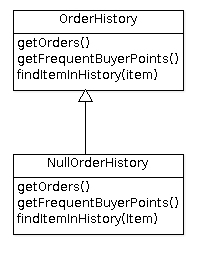
\includegraphics[width=1in]{NullObject.png}

\begin{choices}
\choice Middle Man
\choice Data Clumps
\choice Feature Envy
\choice Parallel Inheritance Hierarchies
\correctchoice Actually, this code is fine
\end{choices}

\question[1] Looking at this class diagram, what is the most significant design problem?

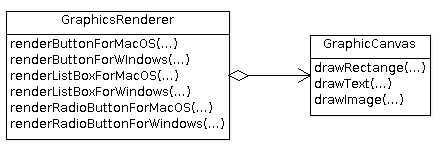
\includegraphics[width=2in]{methodCE.png}

\begin{choices}
\choice The GraphicsRenderer object is a Large Class and some methods should move to GraphicCanvas
\choice The methods of GraphicsRenderer have Feature Envy and should move to GraphicCanvas
\correctchoice The methods of GraphicsRenderer indicate a Combinatorial Explosion
\choice GraphicCanvas and GraphicRenderer should have a common superclass so they can Pull Up common code
\choice Actually, this code is fine
\end{choices}

\question[1] Oftentimes when you refactor a long method with several local variables, you end up with a lot of functions that take many parameters.  Which of these is NOT a good potential solution for this problem?

\begin{choices}
\choice Combine several of the parameters into a new object and pass that instead
\choice Make methods that recompute the variables and call them from each of the functions that need them
\choice Make a new Method Object that contains all the variables and functions related to this computation
\correctchoice Make the parameters instance variables of the class that are null unless the functions are called
\choice All of the choices above are good potential solutions for this problem
\end{choices}

\question[1] Which of these would be an example of divergent change?

\begin{choices}
\correctchoice A FormatParser class that needs to be subclassed in one way when you add a new add format, and another way when you add a new output type
\choice A Sprite class in a video game and that you subclass every time you need a new kind of sprite and implement 3 different abstract methods
\choice A HTTPProtocol class that has one gigantic method that every new feature needs to add to
\choice A web system where you have to both update the C++ backend code as well as the Perl webpage code
\choice A system where everytime you add a new DataElement class, you also need to add a new DataElementRenderer class
\end{choices}

\question[1] Under what circumstances might you want to take two existing classes and give them a common superclass?

\begin{choices}
\correctchoice Both classes have similar methods and you can remove duplication by moving them to the superclass
\choice One class has several Temporary Variables that can be Pulled Up into the superclass
\choice You need to use the superclass as a Middle Man for the clients of both of the classes
\choice Both classes are part of Parallel Inheritance Hierarchies and want to remove the implicit duplcation by giving both hierarchies a shared interface
\choice One class is a Large Class and moving methods into the superclass will make it smaller
\end{choices}

\question[1] What smell does this diagram suggest?

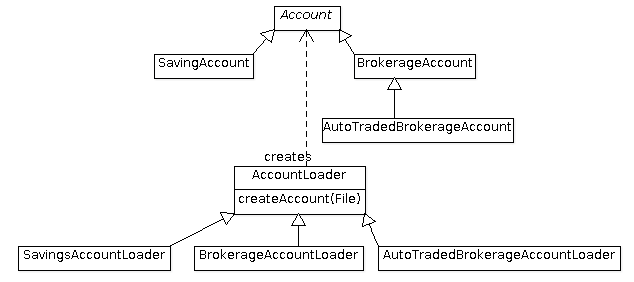
\includegraphics[width=4in]{paralellH.png}

\begin{choices}
\choice Combinatorial Explosion
\choice Middle Man
\choice Refused Bequest
\correctchoice Parallel Inheritance Hierarchies
\choice Actually, this code is fine
\end{choices}

% \question[1] You're reading some code and you come across the class below.  What conclusions do you draw?
% \begin{lstlisting}
% abstract class HTMLTableWriter {
%   public void outputTableHeader() {...}
%   public void outputTableFooter() {...}
%   public abstract void outputTableHeadings();
%   public abstract void outputTableContents();

%   public void outputTable() {
%     outputTableHeader();
%     outputTableHeadings();
%     outputTableContents();
%     outputTableFooter();
%   }
% }

% \end{lstlisting}

% \begin{choices}
% \choice This superclass is an example of Speculative Generality and it's methods should be Pushed Down into it's subclasses
% \choice The method outputTable is probably overridden in HTMLTableWriter's subclasses.  Because HTMLTableWriter is abstract the implementation here can't be called.
% \choice This class could be improved by moving outputTableHeader and outputTableFooter into a newly created class
% \correctchoice The outputTable method is a Template Method
% \choice The outputTable method isn't really accomplishing anything --- it might be worthwhile to use Inline Method on outputTableHeader and outputTableFooter
% \end{choices}

\question[1] You come across the following code.  What refactoring would most improve it?
\begin{lstlisting}
public void updateName(DataRecord newFile) {
  string result = null;
  while(newFile.hasNext()) {
    DataRecordEntry e = newFile.getNext();
    if(e.key().equals("name")) { result = e.value(); }
  }
  if(result == null) throw new RuntimeException("name not found");
  name = result;
}

public void updateName(DataRecord file) {
  string result = null;
  for(DataRecordEntry i = file.getNext(); file.hasNext(); i = file.getNext()) {
    if(i.key().equals("description")) { result = i.value(); }
  }
  if(result == null) throw new RuntimeException("description not found");
  description = result;
}
\end{lstlisting}

\begin{choices}
\correctchoice A single utility method should be extracted and called from both functions, eliminating the duplication
\choice The variables e and i should be renamed to be more explanatory
\choice A local variable should be introduced to explain the method's purpose more clearly
\choice The functions should be changed to return an error code rather than throwing an exception when problems are found
\choice i.key().equals(...) is a Message Chain and should be removed
\end{choices}

\question[1] Object Oriented programmers often say that case statements are bad.  Why?
\begin{choices}
\choice Case statements encourage writing long methods
\choice In languages like Java, strings cannot be used in case statements so they require you to use hard coded constants
\correctchoice Case statements are often vary behavior based on types, which can be replaced by polymorphism
\choice Case statements introduce a strong performance overhead in OO languages because they can't be optimized the same way they can be in procedural languages like C
\choice Case statements often have subtle bugs which more straightforward if statements don't
\end{choices}

\question[1] Imagine you see the following code.  What smell does it suggest?
\begin{lstlisting}
class Person {
  public Person(DatabaseConnection c) {...}
  public Person(NetworkStore c) {...}

  public DatabaseConnection db; //should be null if person was initialized with net
  public NetworkStore net; //should be null if person was initialized with db
  ...
\end{lstlisting}

\begin{choices}
\choice Primitive Obsession
\choice Data Clumps
\choice Divergent Change
\correctchoice Temporary Field
\choice Actually, this code looks fine
\end{choices}

\question[1] Which of these statements most nearly describes how Fowler thinks about comments in code?
\begin{choices}
\choice You should have a comment in the header of every function, but not within the code itself
\correctchoice Comments are not a bad thing, but they can often be made unnecessary by clean code
\choice Comments are useful in procedural languages like C, but not modern languages like Java
\choice Comments are a necessary evil --- we might want our code to be really clean but in real code you generally have to use a lot of comments
\choice Whether or not you use comments is determined by your coding standards, and it's an aesthetic choice that has no effect on your code quality
\end{choices}

\question[1] Imagine you see the following code.  What smell does it suggest?
\begin{lstlisting}
public boolean getsDiscount(Customer customer)
{
  if(customer.isSenior() || customer.isStudent())
    return true;
  if(customer.totalOrderCosts() > FREQUENT_CUSTOMER_CUTOFF)
    return true;
  return false;
}
\end{lstlisting}

\begin{choices}
\choice Duplicate Code
\correctchoice Feature Envy
\choice Middle Man
\choice Temporary Field
\choice Actually, this code is fine
\end{choices}

% \question[1] The code below presents 2 versions of the same function:

% {\em First Version }
% \begin{lstlisting}
% public boolean handleLogfileEntry(String entry) {
%   if(entry.equals("MISSING_RESPONSE")) {
%     missingEntries++;
%     if(missingEntries > MAX_MISSING) doFailedLogfileCheck();
%     return false;
%   } else {
%     Timestamp eventTime = getTimestamp(entry);
%     recordEvent(entry, eventTime);
%     return true;
%   }
% }
% \end{lstlisting}

% {\em Second Version }
% \begin{lstlisting}
% public boolean handleLogfileEntry(String entry) {
%   if(entry.equals("MISSING_RESPONSE")) return handleMissingEntry();

%   Timestamp eventTime = getTimestamp(entry);
%   recordEvent(entry, eventTime);
%   return true;
% }
% \end{lstlisting}

% Is there any reason you might prefer the 1st version to the 2nd?
% \begin{choices}
% \choice The first version puts all the code in one place, which is a good thing
% \correctchoice The first version gives equal weight to both parts of the if clause, which is good if you want to emphasize that missing entries are a normal part of processing
% \choice The first version minimizes function calls, which are likely to have a high performance overhead
% \choice No, the 2nd version is always better
% \end{choices}

% \question[1] What is your reaction to this code?
% \begin{lstlisting}
% List<Student> currentStudents = classRoster.getStudents();
% for(Student student : studentsToRemove) {
%   currentStudents.remove(student);
% }
% \end{lstlisting}
% \begin{choices}
% \choice Functions should not return editable collections
% \choice This code may have unexpected bugs
% \choice A removeStudent method should be added to the classRoster object
% \correctchoice All of the above
% \end{choices}

\question[1] In an error reporting system, you notice a lot of the classes tend to have the same set of 3 instance variables: url, customerId, and timestamp.  What might this suggest?

\begin{choices}
\choice That these three variables often occur together, and should be replaced with a single identifier that links to a global map
\choice That these three variables are a potential source of memory overhead, and you should profile your code to check
\correctchoice That these three objects might be extracted out into a single class
\choice That your classes are likely repeating data and should be combined into one class
\choice That there should be a common superclass of all the classes in the system, and these three fields should be protected members\
\end{choices}


% \question[20]
% Some argue that, ideally, code should be clear even without the presence of comments.  It's definitely true that many of the refactorings we've discussed in class are designed not to change the design of the system, but instead make the code clearer.  These refactorings don't introduce new classes and change inheritance relationships --- instead they make existing classes and functions easier to understand.
% \begin{parts}
%   \part[3] Identify 3 refactorings that have the primary purpose of making things easier to understand
%   \begin{solution}
%     \begin{itemize}
%     \item Rename Method (rename class, rename field)
%     \item Introduce Explaining Variable
%     \item Split Temporary Variable
%     \item Remove Assignments to Parameters
%     \item Replace Array with Object
%     \item some others would probably be reasonable too
%     \end{itemize}
%   \end{solution}
%   \part[7] Write some example code that is difficult to understand, then use at least two of the three refactorings you identified to make a new version of the code the clarifies it.  Be sure it is clear what refactorings you used where.
%   \begin{solution}
% \begin{lstlisting}
% original:

% return computeOutput(student.getEntries());

% refactored:
% double[] studentGrades = student.getEntries();
% return computeWeightedAverage(studentGrades);
% // I used Introduce Explaining Variable to add studentGrades 
% // and Rename Method to change computeOutput
% \end{lstlisting}

%   \end{solution}
%   \part[4] Instead of making the code cleaner, you could usually use comments to document hard--to--understand areas of your code.  Give two reasons why using refactoring might be preferred to detailed code comments.

%   \begin{solution}
%     \begin{itemize}
%     \item Code is more likely to be updated when things change
%     \item Code is easily accessable, comments often require looking up
%       (e.g. a detailed method comment requires going to the class that
%       implements it)
%     \item Making your code clear and broken up often makes it easier
%       to modify (e.g. small methods are easier to override)
%     \end{itemize}
%   \end{solution}
%   \part[6] Some refactorings {\em both} change the structure of the code and make code easier to understand.  Give an example of code (either with UML diagrams or with code itself) before and after a refactoring that changes it's structure and makes it easier to understand.  Include a brief explanation about what about the code is easier to understand now that the refactoring is complete.
% \end{parts}

% \begin{solution}
% \begin{lstlisting}
% original:
% public void computeDistance(double startX, 
%                             double startY, 
%                             double startZ, 
%                             double endX, 
%                             double endY, 
%                             double endZ)

% refactored:
% public void computeDistance(3DPoint start, 3DPoint end)

% // I used Extract Class.  The method is easier to 
% // understand because it makes explict what the 
% // doubles mean and which should be though of as a unit. 
% // Also just reduces the number of parameters you have 
% // to think about.
% \end{lstlisting}
% \end{solution}

\end{questions}
\end{document}


